\documentclass[margin=.5mm]{standalone}
\usepackage[utf8]{inputenc}
\usepackage{tikz}
\usetikzlibrary{calc} 


\begin{document}
    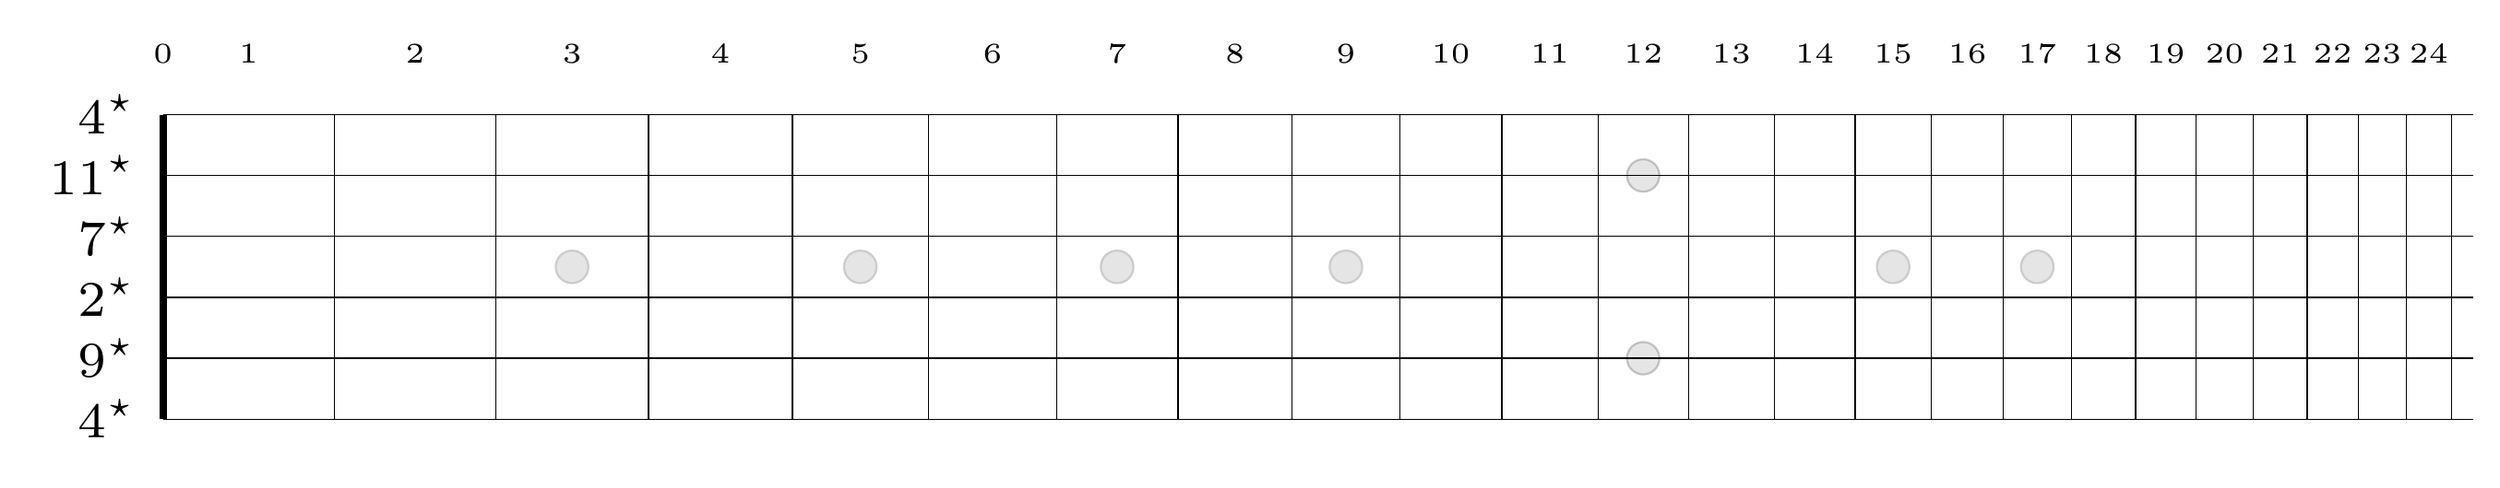
\begin{tikzpicture}[
        ynode/.style={draw=red!50,circle,fill=red!50,scale=.35,inner sep=1pt,minimum size=1.7em}, thick,scale=2.8, every node/.style={scale=2.8}]
    
      %%%% Draw the base and set coordinates %%%%
      \begin{scope}[xscale=-15,yscale=.3,line width=.5]
    
        \xdef\x{1}
        %% Left line
        \draw[line width=3] (1,1) -- (1,6);
        \foreach \fret in {1,...,24}{
          %% Set coordinate for each string
          \foreach \str in {1,...,6}{
            \coordinate (\str-\fret) at (0.97193715634*\x,\str);
          }
          %% Set coordinate for the text above
          \coordinate (Top-\fret) at (0.97193715634*\x,7);
          %% Compute the position of the fret
          \pgfmathsetmacro\x{\x * 0.94387431268}
          \xdef\x{\x}
          %% Draw the fret
          \draw (\x,1) -- (\x,6);
        }
    
        %% Draw each string
        \foreach \str in {1,...,6}{
          \draw (1,\str) -- (0.97153194115*\x,\str);
          \coordinate (start\str) at (1,\str);
        }
        \coordinate (nut) at (1,7);
      \end{scope}
    
      %% Draw the mark on the guitare
      \foreach \f in {3,5,7,9,15,17}{
        \draw[black!20,fill=black!10] ($(3-\f)!.5!(4-\f)$) circle (.08);
      }
      \draw[opacity=.20,fill,fill opacity=.10] (2-12) circle (.08) (5-12) circle (.08);
      
      
      %% DRAWS ALL THE CIRCLES ON IT %%
        %% We define the name of each number
      \newcommand\savename[2]{\expandafter\xdef\csname name#1\endcsname{#2}}
      \newcommand\getname[1]{\csname name#1\endcsname}
      \foreach \n/\t in {1/$9^{\star}$,2/10,3/$11^{\star}$,4/0,5/1,6/$2^{\star}$,7/3,8/$4^{\star}$,9/5,10/6,11/$7^{\star}$,0/8}{
        \savename{\n}{\t}
      }
    
      %% Boucle on the string and the first note (given its number)
      \foreach \str/\note in {1/8,2/1,3/6,4/11,5/3,6/8}{
        \node[anchor=east] at (start\str) {\scriptsize\getname{\note}};
        %\foreach \fret in {1,...,24}{
        %  \pgfmathtruncatemacro\note{mod( \note+1, 12 )}
        %  \xdef\note{\note}
        %  \node[ynode] at (\str-\fret) {\textbf{\getname{\note}}};
        %}
      }
    
      %% Number above each space
      \foreach \fret in {1,...,24}{
        \node[scale=.8] at (Top-\fret) {\tiny \fret};
      }
    \node[scale=.8] at (nut) {\tiny 0};
    
    
    \end{tikzpicture}
\end{document}
